\documentclass[conference]{IEEEtran}
\IEEEoverridecommandlockouts
\usepackage{cite}
\usepackage{comment}
\usepackage{float}
\usepackage{amsmath,amssymb,amsfonts}
\usepackage{algorithmic}
\usepackage{graphicx}
\usepackage{textcomp}
\usepackage{xcolor}
\usepackage{soul}
\usepackage[utf8]{inputenc}
\usepackage[T1]{fontenc}
\usepackage[portuguese]{babel}
\usepackage{booktabs}
\usepackage{hyperref}
\usepackage[export]{adjustbox}

\def\BibTeX{{\rm B\kern-.05em{\sc i\kern-.025em b}\kern-.08em
    T\kern-.1667em\lower.7ex\hbox{E}\kern-.125emX}}

\begin{document}

\title{Viabilidade da Integração de Mobilidade Elétrica na Rede de Distribuição Portuguesa}
\author{
\IEEEauthorblockN{Rui Santiago}
\IEEEauthorblockA{\textit{Dept. de Engenharia Informática} \\
\textit{ISEP}\\
Porto, Portugal \\
1221402@isep.ipp.pt}
\and
\IEEEauthorblockN{Rui Silva}
\IEEEauthorblockA{\textit{Dept. de Engenharia Informática} \\
\textit{ISEP}\\
Porto, Portugal \\
1231105@isep.ipp.pt}
\and
\IEEEauthorblockN{Tiago Barros}
\IEEEauthorblockA{\textit{Dept. de Engenharia Informática} \\
\textit{ISEP}\\
Porto, Portugal \\
1231108@isep.ipp.pt}
}

\maketitle


\begin{abstract}
Este artigo apresenta uma análise exploratória e inferencial da viabilidade técnica de integração de carregadores para veículos elétricos (VE) nos Postos de Transformação de Distribuição (PTD) da rede elétrica portuguesa, com base em dados reais disponibilizados pela e-REDES. A metodologia assenta na quantificação da potência libertada pela substituição de iluminação pública ineficiente (sódio e mercúrio) por tecnologia LED, estimando a folga resultante na rede de baixa tensão. Através de análise exploratória, inferência estatística (testes t, ANOVA) e regressão linear múltipla, avalia-se se a capacidade remanescente é suficiente para suportar carregadores de 22~kW sem comprometer a estabilidade operacional da rede. Os resultados revelam heterogeneidade regional significativa, com o interior do país a apresentar folga substancialmente superior ao litoral, e identificam Lisboa, Porto e Vila Nova de Gaia como os concelhos com maior viabilidade imediata para instalação de infraestrutura de carregamento.
\end{abstract}

\begin{IEEEkeywords}
veículos elétricos, postos de transformação, iluminação pública, eficiência energética, LED, análise exploratória, regressão linear, Portugal
\end{IEEEkeywords}


\section{Introdução e Contextualização}

No contexto da transição energética europeia e da emergência climática, a descarbonização do setor dos transportes e da iluminação urbana tornou-se um imperativo estratégico. Em Portugal, a Iluminação Pública (IP) representa uma fatia expressiva do consumo elétrico municipal, mas a adoção acelerada da tecnologia LED tem demonstrado um potencial disruptivo na libertação de carga na rede de baixa tensão \cite{b1}.

Paralelamente, a expansão da mobilidade elétrica enfrenta o desafio crítico da capacidade da rede. A instalação de pontos de carregamento de VE exige disponibilidade de potência que, em muitas zonas urbanas, já se encontra próxima dos limites operacionais dos PTDs. Surge aqui uma oportunidade de sinergia: a \textit{potência libertada} pela modernização da IP pode constituir o catalisador para a infraestrutura de VE, evitando investimentos massivos em novos PTDs \cite{b5}.

As tempestades que assolaram Portugal no início de 2026, em particular a Tempestade Kristin, evidenciaram a fragilidade da rede elétrica face a picos de carga não planeados, reforçando a necessidade de uma gestão rigorosa da capacidade disponível nos PTDs antes de qualquer expansão de infraestrutura de carregamento.

\subsection{Objetivos}

Os objetivos específicos deste trabalho são: (i)~quantificar a potência libertada pela substituição de tecnologia de IP ineficiente por LED em cada concelho; (ii)~estimar a folga disponível na rede após modernização; (iii)~avaliar estatisticamente a viabilidade técnica de instalação de carregadores de 22~kW por PTD; (iv)~identificar distritos e concelhos com maior potencial de integração de mobilidade elétrica; e (v)~construir um modelo preditivo do nível de ocupação da rede em função das variáveis de infraestrutura.

\subsection{Resumo das Técnicas Estatísticas}

A análise recorre às seguintes técnicas: estatística descritiva; análise de valores omissos e deteção de outliers via boxplot; testes de normalidade de Shapiro-Wilk \cite{b8}; teste $t$ de uma amostra e de duas amostras independentes (variante de Welch); análise de variância de um fator (ANOVA) \cite{b2} com teste post-hoc de Tukey \cite{b9}; correlação de Pearson \cite{b7}; e regressão linear múltipla com diagnóstico de multicolinearidade (VIF) e verificação de pressupostos sobre resíduos através dos testes de Durbin-Watson \cite{b13} e Breusch-Pagan. \cite{b12}

\subsection{Uso de IA generativa}
Em conformidade com o código de conduta desta unidade curricular, importa declarar que o desenvolvimento deste projeto contou com o auxílio de ferramentas de Inteligência Artificial generativa (nomeadamente os modelos Claude Sonnet 4.6 e Gemini 3.1). A sua utilização cingiu-se a um papel de assistente de redação, ajudando a reestruturar e a polir as nossas frases para garantir a adequação do tom e a clareza exigidas num artigo científico rigoroso. Adicionalmente, a IA tomou também um papel apoio durante o desenvolvimento do código e desenvolvimento do \textit{dashboard} interativo. Sublinhamos, contudo, que toda a formulação matemática, o pensamento analítico crítico, as tomadas de decisão na inferência estatística e as conclusões retiradas são da autoria exclusiva e integral do grupo.


\section{Dados e Metodologia}

\subsection{Fontes de Dados}

Os dados provêm da plataforma \textit{open data} da e-REDES \cite{b4}: \texttt{IP\_data.xlsx} com o cadastro da iluminação pública municipal (tipo de lâmpada, potência instalada, código de concelho) e \texttt{PTD\_data.xlsx} com o registo dos PTDs (capacidade nominal em kVA e nível de utilização em intervalos percentuais). O dataset integra 72\,027 PTDs distribuídos por 278 concelhos de Portugal Continental.

Para uma validação da nossa qualidade de dados recorremos também a um \textit{dataset} externo, o "Indicadores de ordenamento do território (Nuts 2024)" com a densidade populacional dos conselhos de Portugal em 2023 e 2024. \cite{b11}

\subsection{Pré-processamento e Engenharia de Variáveis}

Foi criada a variável binária \textit{Is\_Ineficiente} (1 para lâmpadas de sódio ou mercúrio; 0 para outros tipos). O nível de utilização dos PTDs, originalmente em intervalos (e.g., ``60\%--79\%''), foi convertido para valor decimal tomando o limite superior do intervalo. Por agrupamento de concelhos calcularam-se $P\_IP\_Inef$ e $P\_IP\_Total$, a potência gasta em iluminação pública por meios ineficientes e total respetivamente, a capacidade total ($Cap\_PTD$), a utilização média ($Util\_Media$) e o número de PTDs ($N\_PTDs$).

O dataset consolidado integra as seguintes métricas derivadas:
\begin{equation}
\Delta P_{LED} = P\_IP\_Inef \times 0{,}65
\end{equation}
\begin{equation}
P_{Folga} = (Cap\_PTD \times 0{,}92) \times (1 - Util\_Media)
\end{equation}
\begin{equation}
P_{VE} = N\_PTDs \times 22 \times 0{,}60
\end{equation}
\begin{equation}
D = P_{Folga} + \Delta P_{LED} - P_{VE}
\end{equation}
\begin{equation}
Rate\_Ineficiencia = P\_IP\_Inef / P\_IP\_Total
\end{equation}

onde estas representam, respetivamente, a potência libertada num dado concelho pela transição completa para LEDs, a folga existente na rede elétrica de um dado concelho, a potência necessária para instalar carregadores de VEs de 22kW em todos os PTDs de um concelho, a viabilidade técnica desta instalação, com $D > 0$ a indicar viabilidade técnica de integração de VE sem expansão de capacidade instalada, e finalmente, o rácio de ineficiência na iluminação pública de um concelho.


\section{Análise Exploratória de Dados}

\subsection{Mix Tecnológico da Iluminação Pública}

A análise do mix tecnológico, ilustrada na Figura~\ref{fig:3A_1}, revela que, embora se tenha feito muito progresso na otimização da rede de iluminação pública, uma proporção considerativa da potência instalada ainda recorre a tecnologias ineficientes, demonstrando uma clara oportunidade para a libertação de ainda mais potência ao concluir a transição luminotécnica.

\begin{figure}[H]
    \centering
    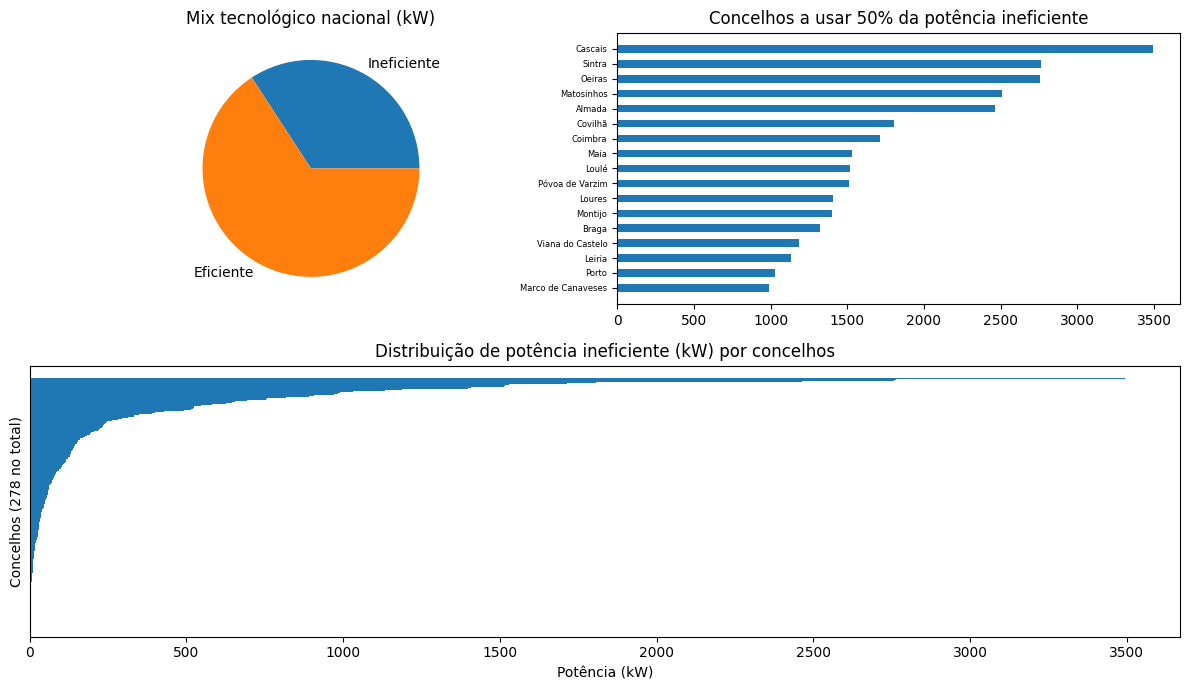
\includegraphics[width=1\linewidth]{img/mix_tec.png}
    \caption{Distribuição da eficiência}
    \label{fig:3A_1}
\end{figure}

Importantemente, uma análise da distribuição geográfica do uso desta potência ineficiente revela que esta encontra-se concentrada num pequeno grupo de concelhos. Só 17 concelhos de um total de 278 ocupam 50\% desta ineficiência.

Estes concelhos são, em larga medida, zonas urbanizadas com uma alta densidade populacional, muitos dos quais parte das áreas metropolitanas do Porto e Lisboa: Isto pode sugerir a potencial futura expansão da infraestrutura de carga de veículos elétricos nestas áreas pode particularmente beneficiar de uma transição luminotécnica completa.

\subsection{Comparação da distribuição dos níveis de utilização entre Lisboa, Porto, Aveiro e Setúbal}
\begin{figure}[H]
    \centering
    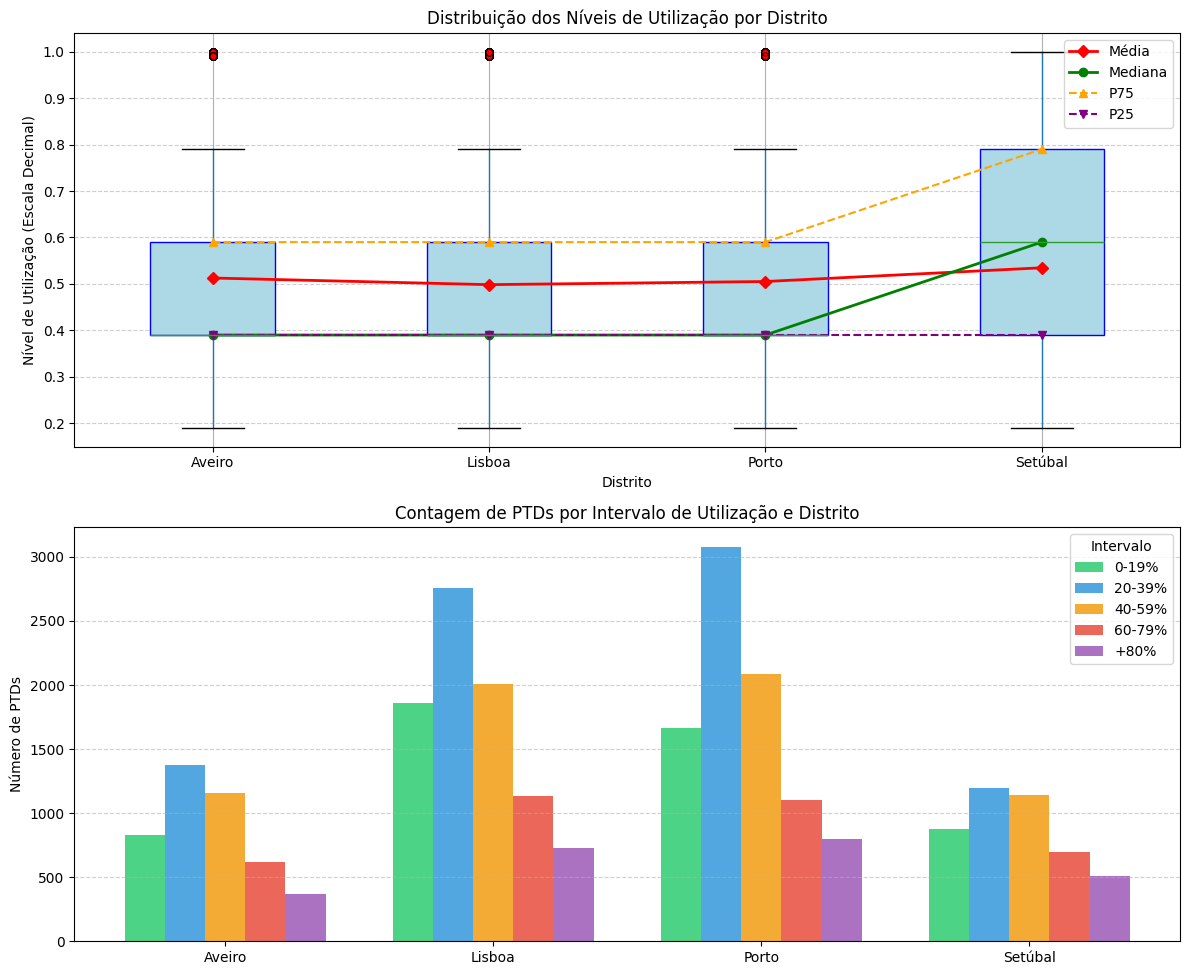
\includegraphics[width=1.0\linewidth]{img/output.png}
    \caption{Boxplot da distribuição dos níveis de utilização e contagem de PTDs por intervalo de utilização}
    \label{fig:3B_1}
\end{figure}
A Figura~\ref{fig:3B_1} apresenta a distribuição dos níveis de utilização dos PTDs para os distritos de Aveiro, Lisboa, Porto e Setúbal. Os quatro distritos apresentam distribuições de níveis de utilização semelhantes, e embora o boxplot sugira uma maior heterogeneidade no concelho de Setúbal, uma análise da distribuição de PTDs em cada concelho de acordo com o seu nível de utilização releva que, na realidade, concelhos como Porto, Lisboa, e em menor grau, Aveiro, contêm uma grande concentração de PTDs com baixos níveis de utilização que não se traduz num menor número de PTDs com alta utilização, refletindo uma rede maioritariamente subcarregada, principalmente nas zonas mais urbanizadas \cite{b4}.

De notar ainda que os valores de Q1, mediana e Q3 tendem a convergir para os limites superiores dos intervalos pré-definidos (0,19; 0,39; 0,59; 0,79), consequência direta da discretização aplicada na conversão dos dados originais \cite{b4}.

\begin{table}[H]
    \caption{Variabilidade de Carga por Distrito (Desvio Padrão Amostral)}
    \begin{center}
    \begin{tabular}{lc}
    \toprule
    \textbf{Distrito} & \textbf{Desvio Padrão ($\sigma$)} \\
    \midrule
    Aveiro  & 0,2379 \\
    Lisboa  & 0,2429 \\
    Porto   & 0,2395 \\
    Setúbal & 0,2540 \\
    \bottomrule
    \end{tabular}
    \label{tab:variabilidade}
    \end{center}
\end{table}

O desvio padrão amostral por distrito é apresentado na Tabela~\ref{tab:variabilidade}. As diferenças entre distritos são modestas, contudo Setúbal regista o valor mais elevado ($\sigma = 0{,}2540$): No entanto, como notado acima, isto não é devido a uma maior heterogeneidade na rede de Setúbal, como pode ser inicialmente assumido. A realidade aparenta simplesmente ser que o número muito mais elevado de PTDs em concelhos como Lisboa e Porto resulta na presença de uma grande quantidade de PTDs com baixa utilização, continuando na mesma a reter níveis semelhantes, até superiores, de PTDs com alta utilização.

Esta análise revela que, para todos estes concelhos, mas em particular para os concelhos de Lisboa e Porto, existe uma grande quantidade de PTDs com baixa utilização que podem ser aproveitados para expandir a infraestrutura de carga de veículos elétricos sem a necessidade de muitas mudanças à rede elétrica atual.

\subsection{Valores Omissos, Indeterminados e Outliers}

\begin{figure}[H]
    \centering
    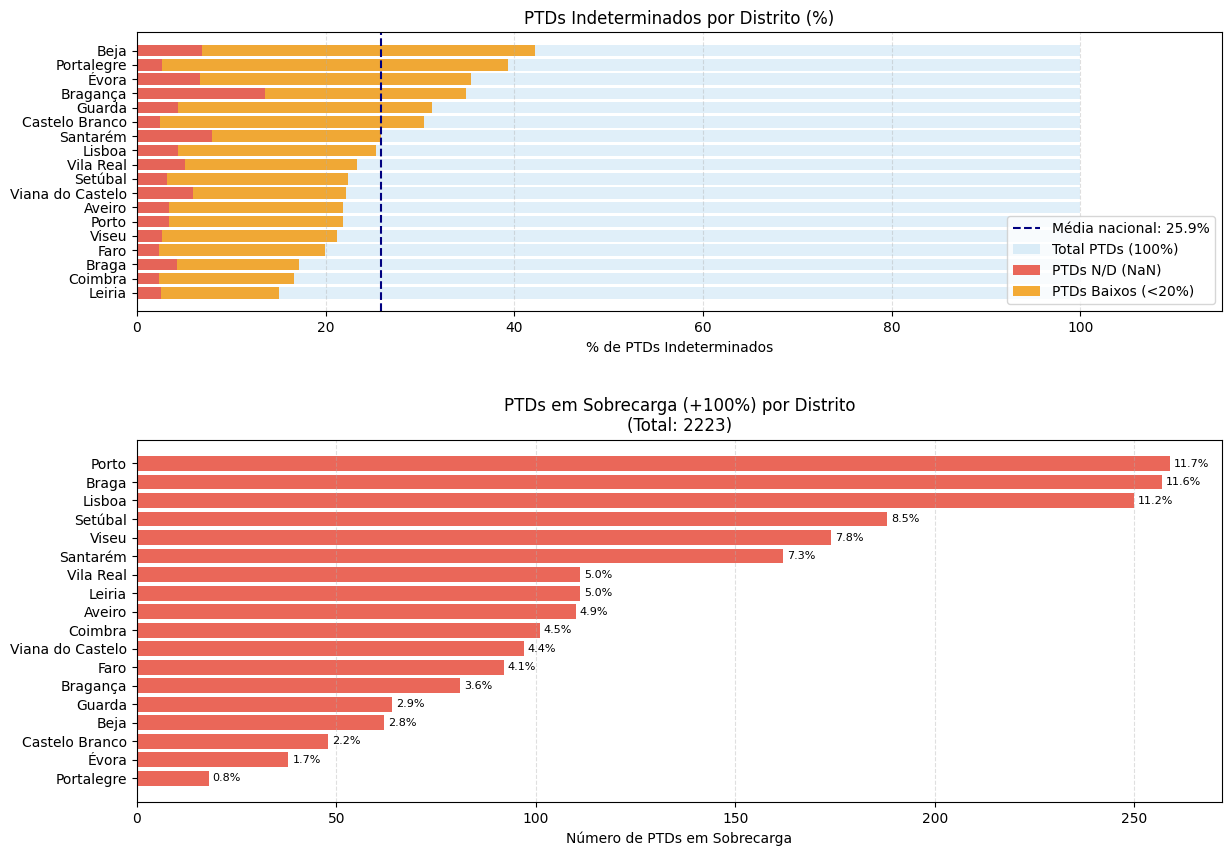
\includegraphics[width=1.0\linewidth]{img/output_3C.png}
    \caption{PTDs indeterminados por distrito (\%) e PTDs em sobrecarga por distrito.}
    \label{fig:3C_1}
\end{figure}

A prevalência de registos omissos e indeterminados é de 25,9\% ao nível nacional. A Fig.~\ref{fig:3C_1} evidencia que esta prevalência não é uniforme, sendo que os distritos do interior como Beja, Portalegre e Évora registam os rácios mais elevados, ultrapassando a média nacional de 25,9\%, ao contrário de Leiria, Coimbra e Braga que se situam abaixo dos 20\%. Esta assimetria é consistente com a menor densidade de infraestrutura de monitorização nas regiões menos urbanizadas \cite{b4}. No entanto, mesmo nas regiões com menos registos omissos e indeterminados, estes continuam a existir em grandes quantidades. Isto sugere que os dados analisados e conclusões interpretadas nas análises deste estudo podem estar a ser afetados por uma falta de dados que pode ser relevante.

Foram identificados 2\,223 PTDs em sobrecarga, correspondendo a 3,09\% da rede. O painel inferior da Fig.~\ref{fig:3C_1} mostra que esta sobrecarga se concentra nos distritos mais populosos como o Porto, Braga e Lisboa, representando em conjunto cerca de um terço do total de PTDs em sobrecarga.

\subsection{Estatísticas Descritivas do Nível de Utilização para Coimbra, Évora, Braga e Faro}

\begin{table}[htbp]
\caption{Estatísticas Descritivas do Nível de Utilização dos PTDs}
\begin{center}
\begin{tabular}{lcccc}
\toprule
\textbf{Estatística} & \textbf{Braga} & \textbf{Coimbra} & \textbf{Évora} & \textbf{Faro} \\
\midrule
Média         & 0,5423 & 0,5406 & 0,4546 & 0,5549 \\
Q1            & 0,39   & 0,39   & 0,19   & 0,39   \\
Mediana       & 0,59   & 0,59   & 0,39   & 0,59   \\
Q3            & 0,79   & 0,79   & 0,59   & 0,59   \\
Desvio Padrão & 0,2401 & 0,2322 & 0,2425 & 0,2126 \\
Assimetria    & 0,4273 & 0,2254 & 0,6659 & 0,2998 \\
Curtose       & -0,7144& -0,7094& -0,4334& -0,4848\\
\bottomrule
\multicolumn{5}{l}{\small Fonte: e-REDES \cite{b4}.}
\end{tabular}
\label{tab:descritiva}
\end{center}
\end{table}

\begin{figure}[H]
    \centering
    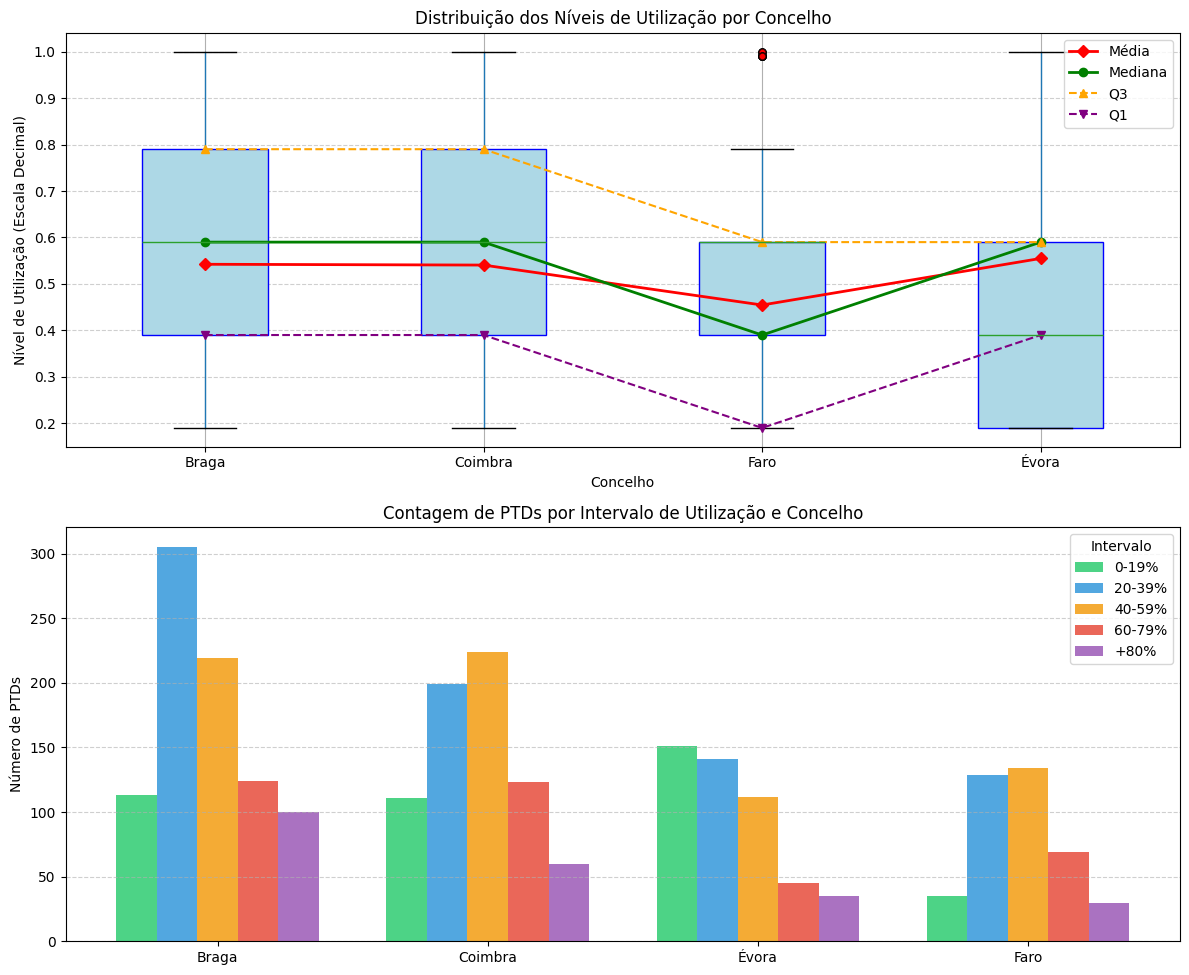
\includegraphics[width=1.0\linewidth]{img/output_3D.png}
    \caption{Distribuição dos níveis de utilização e contagem de PTDs por intervalo 
    para Braga, Coimbra, Évora e Faro.}
    \label{fig:3D_1}
\end{figure}

Évora destaca-se com a média mais baixa (0,4546) e mediana de 0,39, sendo o único concelho onde a maioria dos PTDs opera no intervalo 20--39\%, visível no painel inferior da Fig.~\ref{fig:3D_1}, onde o intervalo 0--19\% é também o mais expressivo relativamente aos restantes concelhos. Faro apresenta a média mais elevada (0,5549) mas o menor desvio padrão (0,2126), sugerindo uma rede mais homogénea. Braga e Coimbra apresentam perfis semelhantes, com o intervalo dominante em 20--39\% e Q3 de 0,79, contrastando com Faro, onde o Q3 desce para 0,59. Todos os concelhos apresentam assimetria positiva e curtose negativa, indicando distribuições platicúrticas com cauda para valores de utilização mais elevados \cite{b1}.

Estas distribuições refletem muito semelhantemente as mesmas analisadas anteriormente para os concelhos de Aveiro, Lisboa, Porto, e Setúbal, com algumas diferenças, nomeadamente a tendência para níveis de utilização extremamente baixos em Évora: As mesmas conclusões dessa análise aplicam-se aqui também.



\section{   Inferência Estatística}
Para a secção de inferência estatística, preparamos três testes de hipótese para conferir se:
\begin{itemize}
  \item Podemos afirmar que o nível médio de ocupação da rede é inferior a um patamar de referência, que foi decidido ser de 60\%.
  \item Podemos afirmar que o nível médio de ocupação da rede difere significativamente entre concelhos modernizados (rácio LED acima da mediana) e ineficientes.
  \item Podemos afirmar que existem diferenças significativas no nível médio de ocupação da rede entre três regiões: Norte/Centro Litoral, Lisboa e Litoral Sul, e Interior/Alentejo.
\end{itemize}

Todos os testes foram realizados com um nível de significância $\alpha = 0{,}05$.

Utilizaram-se amostras selecionadas aleatoriamente; os valores do $p-value$ e da estatística $t$ apresentados baseiam-se numa \textit{seed} fixa de 32. A normalidade das amostras foi previamente verificada através do teste de Shapiro-Wilk \cite{b8}. 

Para garantir a robustez dos resultados, cada teste foi validado num intervalo de \textit{seeds} de 1 a 100, verificando-se a respetiva taxa de aceitação.

\subsection{Teste ao Nível Médio de Ocupação da Rede}

Selecionou-se aleatoriamente uma amostra de 50 concelhos. O teste de Shapiro-Wilk confirmou a normalidade da amostra ($W = 0{,}978$, $p = 0{,}484$). Aplicou-se o teste $t$ de uma amostra com hipótese unilateral:
\begin{equation}
H_0: \mu \geq 0{,}60 \quad \text{vs} \quad H_1: \mu < 0{,}60
\end{equation}

O resultado ($\bar{x} = 0{,}505$, $t = -11{,}47$, $p < 0{,}001$) leva à rejeição de $H_0$, concluindo-se que a ocupação média da rede é significativamente inferior ao patamar de 60\%. Este resultado sugere que existe, em geral, capacidade disponível nos PTDs portugueses. A robustez desta conclusão foi validada através de 100 sementes distintas: $H_0$ foi rejeitado em 86\% dos casos, com 14\% das sementes a produzir amostras que não satisfizeram o pressuposto de normalidade.

\subsection{Comparação entre Concelhos Modernizados e Ineficientes}

Foram selecionadas aleatoriamente duas amostras de 30 concelhos cada: ``Modernizados'' ($Rate\_Inef \leq$ mediana) e ``Ineficientes'' ($Rate\_Inef >$ mediana). Ambas as amostras satisfizeram o pressuposto de normalidade (Shapiro-Wilk: $p = 0{,}357$ e $p = 0{,}365$, respetivamente) e de homocedasticidade (Levene \cite{b14}: $p = 0{,}502$). O teste $t$ de Welch para duas amostras independentes avalia:
\begin{equation}
H_0: \mu_{mod} = \mu_{inef} \quad \text{vs} \quad H_1: \mu_{mod} \neq \mu_{inef}
\end{equation}

O resultado ($\bar{x}_{mod} = 0{,}503$, $\bar{x}_{inef} = 0{,}513$, $t = -0{,}518$, $p = 0{,}607$) não permite rejeitar $H_0$. Conclui-se que a transição para LED, embora liberte potência localizada, não altera de forma estatisticamente significativa o perfil médio de ocupação macro dos PTDs. Numa análise de 100 sementes, $H_0$ foi rejeitado em apenas 28\% dos casos, com 27\% a não satisfazer normalidade, reforçando a robustez desta conclusão.

\subsection{ANOVA: Perfis Regionais de Ocupação}

Foram constituídas três amostras de 25 concelhos representativas de perfis regionais distintos: Norte/Centro Litoral (Porto, Braga, Coimbra), Lisboa e Litoral Sul (Lisboa, Setúbal, Aveiro) e Interior/Alentejo (Évora, Beja, Portalegre). Verificados os pressupostos de normalidade (Shapiro-Wilk: $p > 0{,}22$ nos três grupos) e homocedasticidade (Levene: $p = 0{,}552$), a ANOVA de um fator \cite{b2} revelou diferenças altamente significativas ($F = 26{,}16$, $p < 0{,}001$).

A análise post-hoc de Tukey \cite{b9} (Tabela~\ref{tab:tukey}) identificou que o Interior/Alentejo ($\bar{x} = 0{,}427$) difere significativamente de ambas as regiões litorais (Lisboa/Litoral Sul: $\bar{x} = 0{,}513$, $p < 0{,}001$; Norte/Centro: $\bar{x} = 0{,}538$, $p < 0{,}001$), não existindo diferença significativa entre as duas regiões litorais ($p = 0{,}265$). Esta robustez foi confirmada em 100 sementes, com $H_0$ rejeitado em 70\% dos casos.

\begin{table}[htbp]
\caption{Análise Post-hoc de Tukey -- Comparação Regional}
\begin{center}
\begin{tabular}{llccc}
\toprule
\textbf{Grupo 1} & \textbf{Grupo 2} & \textbf{Dif. Médias} & $p_{adj}$ & \textbf{Rejeita} \\
\midrule
Interior     & Lisboa/Litoral & 0.0858 & $<$0.001 & Sim \\
Interior     & Norte/Centro   & 0.1111 & $<$0.001 & Sim \\
Lisboa/Lit.  & Norte/Centro   & 0.0253 & 0.265    & Não \\
\bottomrule
\end{tabular}
\label{tab:tukey}
\end{center}
\end{table}

\subsection{Correlação entre Capacidade de Transformação e Carga de IP}

O coeficiente de Pearson \cite{b7} entre $Cap\_PTD$ e $P\_IP\_Total$ para a totalidade dos concelhos revelou uma correlação muito forte e positiva ($r = 0{,}911$, $p < 0{,}001$), rejeitando $H_0: \rho = 0$. Elevando ao quadrado, $r^2 \approx 0{,}83$, indicando que 83\% da variabilidade da carga de IP é explicada pela capacidade instalada dos PTDs. Esta forte colinearidade era expectável, refletindo o dimensionamento da rede em função da dimensão urbana de cada município, e tem implicações diretas na multicolinearidade do modelo preditivo.


\section{Correlação, Regressão e Modelo Preditivo}

\subsection{Modelo de Regressão Linear Múltipla}

Para analisar a variação do estado de ocupação médio da rede, foi ajustado um modelo de regressão linear múltipla utilizando o método dos Mínimos Quadrados Ordinários (OLS). A amostra incidiu sobre 64 concelhos pertencentes aos distritos de Aveiro, Braga, Lisboa e Porto.

A variável dependente ($Y$) definida foi o Nível Médio de Utilização, sendo explicada pelas seguintes variáveis independentes: Potência Instalada Total de IP ($X_1$), Capacidade Nominal de Transformação ($X_2$) e o Rácio de Ineficiência ($X_3$). 

Os resultados detalhados da regressão encontram-se sumarizados na Tabela~\ref{tab:regressao_multipla}.

\begin{table}[H]
\caption{Resultados do Modelo de Regressão Linear Múltipla}
\begin{center}
\begin{tabular}{lcccc}
\toprule
\textbf{Variável} & $\hat{\beta}$ & \textbf{Erro Padrão} & $t$ & $p$-value \\
\midrule
Intercepto ($\beta_0$)  & 0,5417    & 0,010    & 54,323 & $<$0,001 \\
$X_1$  & 1,733e-05 & 1,29e-05 & 1,340  & 0,185    \\
$X_2$      & -1,949e-07& 6,69e-08 & -2,914 & 0,005    \\
$X_3$   & 0,0131    & 0,031    & 0,426  & 0,672    \\
\bottomrule
\multicolumn{5}{l}{\small $R^2 = 0{,}276$\quad $R^2_{adj} = 0{,}240$\quad $F = 7{,}63$\quad $p = 0{,}0002$}
\end{tabular}
\label{tab:regressao_multipla}
\end{center}
\end{table}

Relativamente à contribuição individual de cada preditor, avaliada ao mesmo nível de significância ($\alpha = 0{,}05$), verifica-se que apenas a Capacidade Nominal do PTD ($X_2$) apresenta um efeito estatisticamente significativo ($p = 0{,}005$). O seu coeficiente negativo ($\hat{\beta}_2 = -1{,}949 \times 10^{-7}$) indica que postos com maior capacidade tendem a apresentar menores taxas de ocupação, como seria expectável. Em contrapartida, as variáveis referentes à Potência Instalada de IP ($X_1$, $p = 0{,}185$) e ao Rácio de Ineficiência ($X_3$, $p = 0{,}672$) não se revelaram preditores estatisticamente significativos para a ocupação média da rede. A falta de significância de $X_1$ pode ser parcialmente explicada pela forte multicolinearidade com $X_2$ (concelhos com maior capacidade instalada tendem a ter maior potência de IP), enquanto o resultado de $X_3$ sugere que o nível de ineficiência tecnológica da iluminação, de forma isolada, não dita o estado de saturação macro da rede elétrica.

\subsection{Verificação dos Pressupostos do Modelo}

A validade da inferência estatística do modelo de regressão linear múltipla depende do cumprimento rigoroso das condições dos resíduos. A avaliação foi conduzida conjugando testes de hipóteses formais e diagnóstico gráfico.

\subsubsection{Normalidade dos Resíduos}
Para verificar a normalidade dos erros, formulou-se o teste de Shapiro-Wilk \cite{b8}:
\begin{center}
    $H_0$: Os resíduos seguem uma distribuição normal. \\
    $H_1$: Os resíduos não seguem uma distribuição normal.
\end{center}
A estatística de teste obtida foi $W = 0{,}9795$ com um $p\text{-value} = 0{,}3646$. Sendo $p > \alpha$ (para um nível de significância $\alpha = 0{,}05$), não se rejeita a hipótese nula ($H_0$). Conclui-se que a condição de normalidade está satisfeita, facto corroborado pelo Gráfico Quantil-Quantil (Figura~\ref{fig:qq_plot}), onde os resíduos se alinham de forma consistente sobre a diagonal teórica, sem desvios acentuados nas extremidades.

\begin{figure}[H]
    \centering
    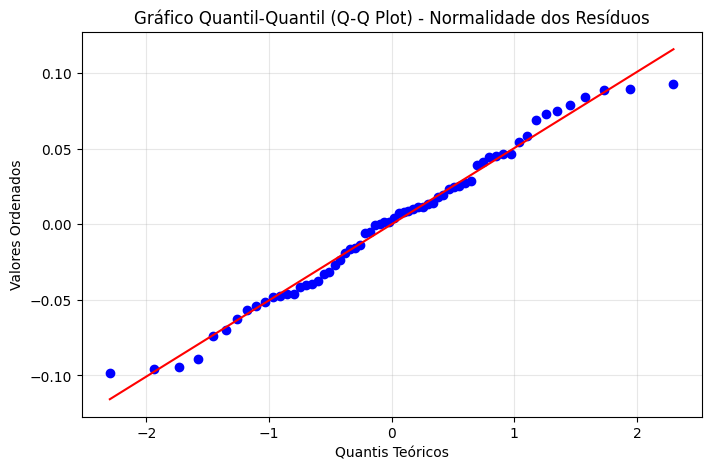
\includegraphics[width=0.9\linewidth]{img/qq_plot.png}
    \caption{Gráfico Quantil-Quantil (Q-Q Plot) para Avaliação da Normalidade}
    \label{fig:qq_plot}
\end{figure}

\subsubsection{Independência}
Para garantir a ausência de autocorrelação nos resíduos, aplicou-se o teste de Durbin-Watson \cite{b15}:
\begin{center}
    $H_0$: Ausência de autocorrelação (resíduos independentes). \\
    $H_1$: Existência de autocorrelação entre os resíduos.
\end{center}
O teste devolveu a estatística $DW = 1{,}8805$. Encontrando-se este valor muito próximo de 2 (limiar de ausência de correlação), não se rejeita $H_0$, provando-se que os erros de previsão de um concelho não estão estatisticamente associados aos concelhos vizinhos.

\subsubsection{Homocedasticidade}
A constância da variância dos erros (homocedasticidade) foi avaliada através do diagnóstico gráfico de dispersão dos resíduos face aos valores previstos (Figura~\ref{fig:res_vs_fit}). 
A distribuição dos pontos apresenta-se globalmente aleatória em torno do eixo horizontal (zero), não se identificando qualquer padrão geométrico de afunilamento (forma de cone ou funil) que sugerisse um aumento ou diminuição sistemática da variância. Isto confirma que a margem de erro do modelo se mantém estável, encontrando-se o pressuposto plenamente assegurado.

\begin{figure}[H]
    \centering
    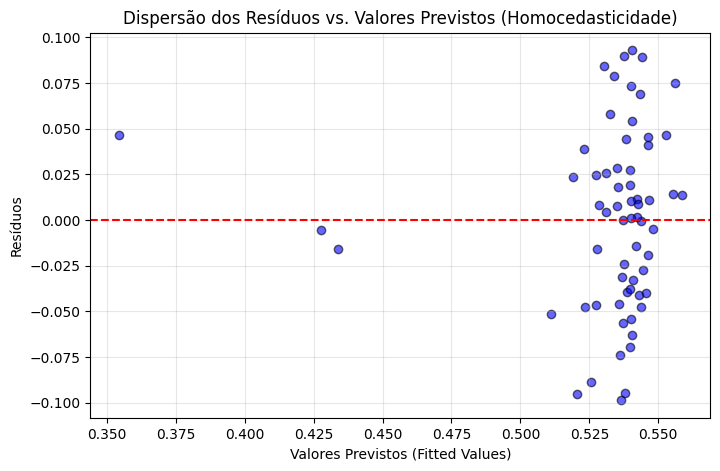
\includegraphics[width=0.9\linewidth]{img/residuos_vs_ajustados.png}
    \caption{Dispersão dos Resíduos vs. Valores Previstos (Homocedasticidade)}
    \label{fig:res_vs_fit}
\end{figure}

\subsection{Diagnóstico de Multicolinearidade}

A presença de multicolinearidade entre as variáveis preditoras foi avaliada através do Fator de Inflação da Variância (VIF). Os resultados obtidos foram os seguintes:

\begin{itemize}
    \item $X_1$ (Potência Instalada de IP): $VIF = 8{,}39$
    \item $X_2$ (Capacidade do PTD): $VIF = 7{,}53$
    \item $X_3$ (Rácio de Ineficiência): $VIF = 1{,}44$
\end{itemize}

Observa-se multicolinearidade (VIF > 5) entre a Potência Instalada ($X_1$) e a Capacidade Nominal ($X_2$). Este resultado era estritamente expectável e reflete o desenho estrutural da rede: concelhos com maior dimensão urbana possuem, em simultâneo, maior potência de iluminação e postos com maior capacidade. 

O Rácio de Ineficiência ($X_3$) apresenta um VIF próximo de 1, indicando total ausência de colinearidade com as restantes variáveis.

A multicolinearidade moderada entre $X_1$ e $X_2$ justifica o facto de o preditor $X_1$ ter perdido a sua significância estatística individual ($p = 0{,}185$) no modelo.

\subsection{Estimação e Intervalos de Confiança (Distrito de Aveiro)}

Com o intuito de validar a aplicabilidade prática do modelo, efetuou-se a previsão do nível de ocupação ($Y$) para os nove concelhos do distrito de Aveiro. As estimativas não foram tratadas como valores pontuais exatos, mas sim acompanhadas do cálculo do respetivo intervalo de Confiança (IC) a 95\% para novas observações.

Os resultados numéricos extraídos constam da Tabela~\ref{tab:aveiro_ic} e a sua representação visual é ilustrada na Figura~\ref{fig:aveiro_ic}.

\begin{table}[htbp]
\caption{Previsões e Intervalos de Confiança a 95\% (Aveiro)}
\begin{center}
\begin{tabular}{ccccc}
\toprule
\textbf{Cód.} & \textbf{$Y$ Real} & \textbf{Prev. ($\hat{Y}$)} & \textbf{Lim. Inf.} & \textbf{Lim. Sup.} \\
\midrule
101 & 0,4776 & 0,5404 & 0,4379 & 0,6429 \\
102 & 0,4699 & 0,5398 & 0,4367 & 0,6428 \\
103 & 0,5430 & 0,5438 & 0,4408 & 0,6467 \\
104 & 0,5274 & 0,5463 & 0,4436 & 0,6490 \\
105 & 0,4755 & 0,5233 & 0,4206 & 0,6260 \\
106 & 0,5432 & 0,5481 & 0,4451 & 0,6512 \\
107 & 0,4434 & 0,5379 & 0,4350 & 0,6407 \\
108 & 0,5076 & 0,5408 & 0,4378 & 0,6437 \\
109 & 0,5829 & 0,5385 & 0,4353 & 0,6416 \\
\bottomrule
\end{tabular}
\label{tab:aveiro_ic}
\end{center}
\end{table}

\begin{figure}[H]
    \centering
    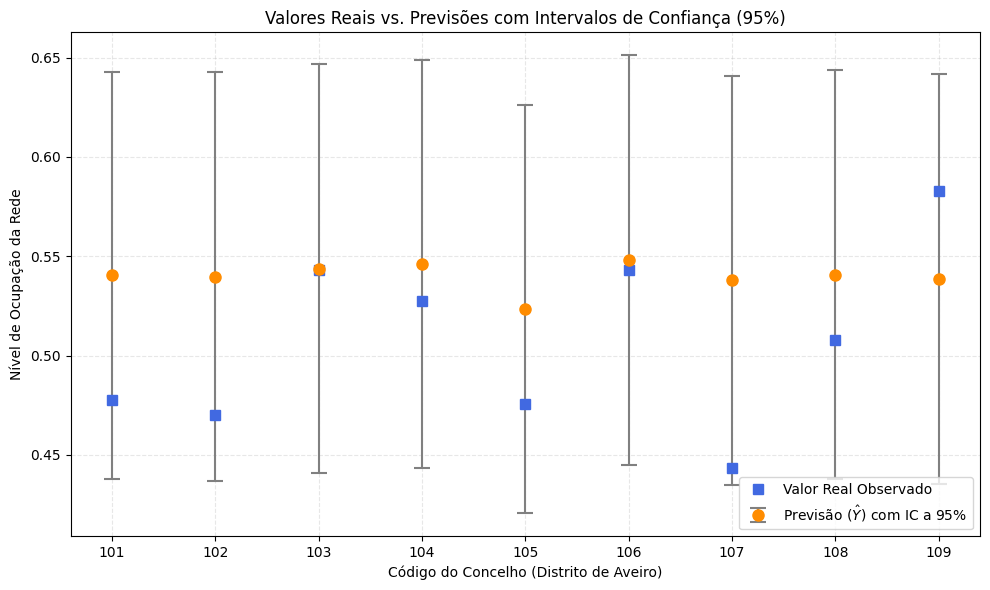
\includegraphics[width=0.9\linewidth]{img/ic_aveiro.png}
    \caption{Valores Reais face aos Intervalos de Confiança a 95\% das Previsões}
    \label{fig:aveiro_ic}
\end{figure}

A análise gráfica e tabular revela um resultado notável: todos os 9 valores reais de ocupação observados (100\% da amostra de teste) recaem estritamente dentro dos limites do Intervalo de Confiança a 95\% gerado pelo modelo. Este facto corrobora a adequação do modelo linear múltiplo ajustado. 

Demonstra-se assim que, apesar do coeficiente de determinação evidenciar a existência de variância não explicada, as fronteiras de previsão são estatisticamente sólidas e englobam com precisão a variabilidade real operacional da rede elétrica de distribuição.

\subsection{Simulação de Impacto: Redução da Ineficiência Tecnológica}

Com o modelo validado, procedeu-se à quantificação prática do impacto da modernização da infraestrutura. Utilizando o coeficiente estimado para a variável de ineficiência ($\hat{\beta}_3 = 0{,}0131$), simulou-se um cenário em que a percentagem de lâmpadas ineficientes na rede sofria uma redução de 20\% ($\Delta X_3 = -0{,}20$).

\begin{comment}
A redução esperada no nível médio de ocupação da rede ($\Delta \hat{Y}$) é dada por:
$$
\Delta \hat{Y} = \hat{\beta}_3 \times \Delta X_3 = 0{,}0131 \times (-0{,}20) = -0{,}00262
$$
\end{comment}

A projeção matemática demonstra que uma forte transição de 20\% para tecnologia LED resultaria numa redução de ocupação média de apenas 0,263 pontos percentuais. Esta conclusão reforça e traduz estatisticamente a inferência central deste estudo: a libertação de potência gerada pela eficientização da iluminação pública, embora tecnicamente existente, tem uma magnitude negligenciável e não altera o paradigma de viabilidade estrutural dos PTDs.

\subsection{Identificação de Concelhos Prioritários para VE}

Para identificar os concelhos mais viáveis para instalação de carregadores VE (22~kW), filtrou-se por $D > 0$ e ordenou-se pelo Saldo de Viabilidade em ordem decrescente; o critério mais direto para responder à questão central: após instalar os carregadores e substituir a iluminação ineficiente, a rede aguenta? A Tabela~\ref{tab:top10_ve} apresenta o Top 10.

\begin{table}[htbp]
\caption{Top 10 Concelhos para Instalação de Carregadores VE (22~kW)}
\begin{center}
\begin{tabular}{lccc}
\toprule
\textbf{Concelho} & \textbf{Saldo (kVA)} & \textbf{Ocup. Prev.} & \textbf{Lim. Sup. 95\%} \\
\midrule
Lisboa            & 944\,820 & 0,3543 & 0,4855 \\
Porto             & 431\,041 & 0,4276 & 0,5478 \\
V. N. de Gaia     & 391\,919 & 0,4339 & 0,5479 \\
Sintra            & 211\,284 & 0,5353 & 0,6520 \\
Cascais           & 204\,317 & 0,5397 & 0,6505 \\
Matosinhos        & 201\,909 & 0,5255 & 0,6325 \\
Oeiras            & 186\,489 & 0,5361 & 0,6431 \\
Maia              & 183\,148 & 0,5207 & 0,6254 \\
Gondomar          & 149\,137 & 0,5110 & 0,6146 \\
Braga             & 146\,730 & 0,5190 & 0,6226 \\
\bottomrule
\end{tabular}
\label{tab:top10_ve}
\end{center}
\end{table}

Lisboa lidera com 944\,820~kVA de saldo e ocupação prevista de apenas 35,4\%. O Top 10 é dominado por concelhos das duas áreas metropolitanas, consistente com os resultados da ANOVA; regiões litorais com maior capacidade instalada e, consequentemente, maior folga para absorver carga VE.


\section{Análise e Discussão de Resultados}
Os dados revelam que a ineficiência tecnológica está altamente concentrada, com metade da potência ineficiente nacional restrita a apenas 17 concelhos. Contudo, a análise inferencial sugere que esta concentração não se traduz numa oportunidade proporcional para a mobilidade elétrica de média potência.

O teste $t$ de Welch ($p = 0,607$) não permitiu distinguir o nível médio de ocupação entre concelhos "Modernizados" e "Ineficientes". Este resultado é corroborado pela quantificação direta da potência libertada: o ganho mediano por PTD (2-3~kW) representa apenas um incremento de \textbf{1,1\%} a \textbf{1,5\%} face aos 22~kW requeridos.

A Fig.~\ref{fig:6_1} abaixo ilustra a percentagem de potência libertada, para cada distrito, que uma transição luminotécnica completa traria: Até no caso mais impactante, só existe um aumento de pouco mais que 1\%. O ponto central aqui é que, embora a modernização reduza o consumo, a sua escala é insuficiente para alterar o estado de viabilidade técnica de um posto saturado.

\begin{figure}[H]
    \centering
    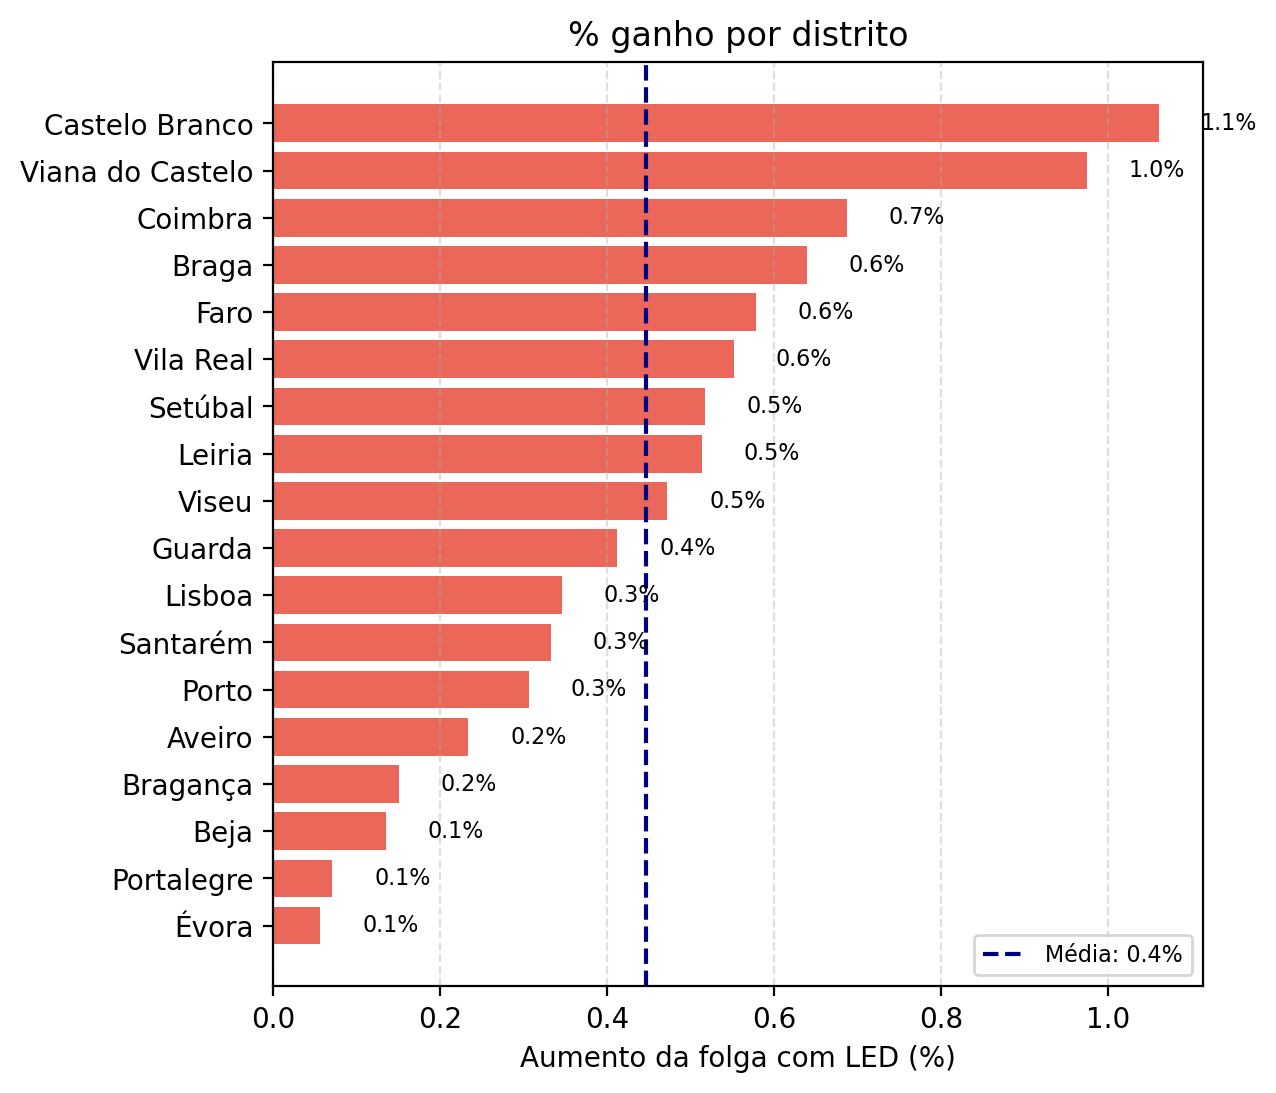
\includegraphics[width=1\linewidth]{img/potencia_libertada.png}
    \caption{Distribuição do ganho por distrito}
    \label{fig:6_1}
\end{figure}

\subsection{Dinâmica Regional e Variabilidade de Carga}

A aplicação da ANOVA confirmou disparidades regionais estatisticamente significativas ($F = 26,16$, $p < 0,001$). O Interior e o Alentejo apresentam, de forma consistente, níveis de ocupação inferiores ($\bar{x} = 0,427$) em comparação com as zonas litorais. 

No entanto, a correlação de Pearson ($r = 0,911$) indica que o dimensionamento da rede acompanha estritamente a dimensão urbana. O que podemos inferimos disto é que a folga superior no interior resulta de uma menor densidade de carga base e não necessariamente de uma gestão de eficiência mais agressiva do que no litoral.

\begin{figure}[H]
    \centering
    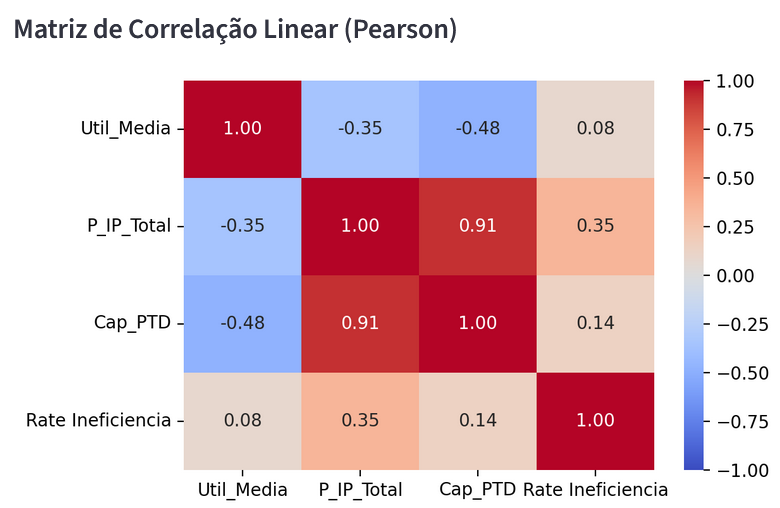
\includegraphics[width=1\linewidth]{img/matriz_pearson.png}
    \caption{Matriz de correlação de Pearson para as variáveis de carga e métricas urbanas regionais}
    \label{fig:placeholder}
\end{figure}

\subsection{Eficácia do Modelo Preditivo}

O modelo de regressão múltipla revelou que apenas a capacidade nominal do PTD ($X_2$) possui um efeito estatisticamente significativo na ocupação ($p = 0,005$). O rácio de ineficiência ($X_3$) revelou-se um preditor nulo neste contexto ($p = 0,672$).

Com um $R^2_{adj} = 0,240$, o modelo sugere que a ocupação da rede de baixa tensão é governada por variáveis exógenas não incluídas no mix tecnológico da iluminação, como o consumo doméstico sazonal ou atividade comercial. O que nos dá a entender que a modernização da iluminação pública, isoladamente, explica uma fração negligenciável da dinâmica de carga da rede.

\subsection{Impacto de Falta de Dados}

\begin{figure}[H]
    \centering
    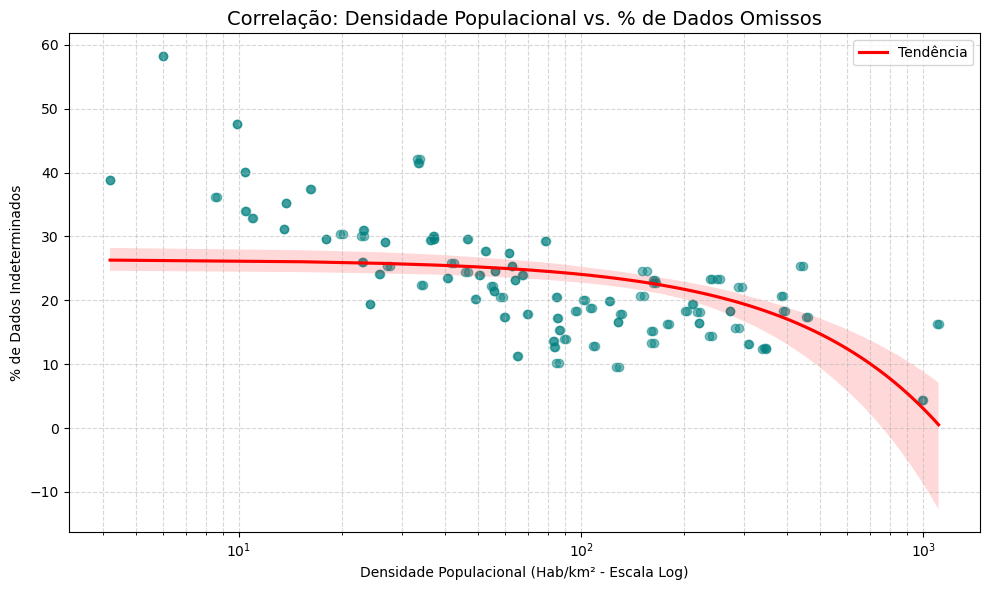
\includegraphics[width=1\linewidth]{img/dpvsdo.png}
    \caption{Relaçao entre concelhos com dados omissos e a sua densidade populacional}
    \label{fig:4_C}
\end{figure}

A relação entre os dados omissos e a densidade populacional dos concelhos (Fig. ~\ref{fig:4_C}) revela um problema crítico: a omissão de dados, que pode ser um problema particularmente importante em zonas de alta densidade. Embora a média de falhas seja transversal ao território, ter quase 20\% de dados em falta em grandes centros urbanos gera uma 'cegueira' operacional onde a procura de VE é maior.

\subsection{Condições Pré-existentes}

Embora as conclusões principais deste estudo tenham indicado que a continuação da modernização das redes de iluminação pública não tenha uma impacto significante na viabilidade técnica da expansão da infraestrutura de carregamento de veículos elétricos, é também importante notar como também se pode concluir das análises conduzidas que a rede elétrica atual já consegue facilmente suportar essa expansão.

Como foi ilustrado nas análises dos níveis de utilização atuais de PTDs em diversos concelhos (Figs. ~\ref{fig:3B_1} e ~\ref{fig:3D_1}), a rede elétrica atual aparenta ser, em larga medida, subcarregada e com uma grande folga que pode ser aproveitada para a carga de VEs, particularmente em centros urbanos como Lisboa e Porto. Não existe necessidade de esperar por uma modernização completa da iluminação pública para começar esta expansão.


\section{Conclusão}

O presente estudo demonstrou que a substituição da iluminação pública tradicional por tecnologia LED, embora relevante para a eficiência energética e redução de custos operacionais, tem um impacto marginal na expansão da infraestrutura de mobilidade elétrica. No entanto, também demonstrou que a rede elétrica atual já disponibiliza, em larga medida, a potência livre necessária para essa expansão, devido à grande quantidade de PTDs com baixos níveis de utilização que podem ser aproveitados para esta tarefa.

É também importante notar que isto também significa que uma expansão ainda mais extensiva da infraestrutura de carga de VEs irá depender do reforço adicional da rede elétrica, e não da otimização da mesma através da modernização luminotécnica: Um reforço que será, sem dúvida, eventualmente necessário à medida que a descarbonização e eletrificação dos transportes civis portugueses continua.

\begin{thebibliography}{00}

\bibitem{b1}
C. Heumann e M. Schomaker, \textit{Introduction to Statistics and Data Analysis}. Springer International Publishing, 2016.

\bibitem{b2}
D. C. Montgomery, \textit{Design and Analysis of Experiments}, 8.ª ed. John Wiley \& Sons, New York, 2013.

\bibitem{b3}
W. McKinney, \textit{Python for Data Analysis: Data Wrangling with Pandas, NumPy, and Jupyter}, 3.ª ed. O'Reilly Media, 2022. [Online]. Disponível em: \url{https://wesmckinney.com/book/}

\bibitem{b4}
e-REDES, ``Open Data -- Postos de Transformação de Distribuição,'' [Online]. Disponível em: \url{https://e-redes.opendatasoft.com/pages/homepage/}

\bibitem{b11}
INE, ``Base Dados, Densidade populacional (N.º/ km²) por Local de residência (NUTS - 2024),'' [Online]. Disponível em: \url{https://censos.ine.pt/xportal/xmain?xpid=INE&xpgid=ine_indicadores&userLoadSave=Load&userTableOrder=13050&tipoSeleccao=1&contexto=pq&selTab=tab1&submitLoad=true&xlang=pt}

\bibitem{b5}
Agência Portuguesa do Ambiente, ``Estratégia Nacional para a Mobilidade Elétrica,'' Lisboa, 2023.

\bibitem{b7}
K. Pearson, ``Notes on regression and inheritance in the case of two parents,'' \textit{Proceedings of the Royal Society of London}, vol. 58, pp. 240--242, 1895.

\bibitem{b8}
S. S. Shapiro e M. B. Wilk, ``An analysis of variance test for normality (complete samples),'' \textit{Biometrika}, vol. 52, n.º 3/4, pp. 591--611, 1965.

\bibitem{b9}
J. W. Tukey, \textit{Exploratory Data Analysis}. Addison-Wesley, 1977.

\bibitem{b10}
R. E. Walpole, R. H. Myers e S. L. Myers, \textit{Probability and Statistics for Engineers and Scientists}, 9.ª ed. Pearson, 2012.

\bibitem{b12}
T. S. Breusch e A. R. Pagan, ``A simple test for heteroscedasticity and random coefficient variation,'' \textit{Econometrica}, vol. 47, n.º 5, pp. 1287--1294, 1979.

\bibitem{b13}
J. Durbin e G. S. Watson, ``Testing for serial correlation in least squares regression,'' \textit{Biometrika}, vol. 38, n.º 1/2, pp. 159--177, 1951.

\bibitem{b14}
H. Levene, ``Robust tests for equality of variances,'' in \textit{Contributions to Probability and Statistics}, I. Olkin et al., Eds. Stanford University Press, 1960, pp. 278--292.

\bibitem{b15}
J. Durbin e G. S. Watson, ``Testing for Serial Correlation in Least Squares Regression: I,'' \textit{Biometrika}, vol. 37, n.º 3/4, pp. 409--428, 1950.

\end{thebibliography}

\end{document}
